% Manuel Lippert - Paul Schwanitz
% Physikalisches Praktikum

% Auswertung Teil 1

\section{invertierteres Pendel}
\label{sec:auswertungPendel}

\subsection{Bifurkationsdiagramm und kritische Masse}
\label{sub:bifuAndKritMass}
Über den Versuch wurde die Auslenkung $\theta$ bzw. die Spannung $U_a$ am Digitalmultimeter links ($U_{a,l}$) und rechts ($U_{a,r}$) gemessen. Dabei ergeben sich erst ab einer gewissen Masse, eine Auslenkung links oder rechts, was im Bifurkationsdiagramm (Abb \ref{image:bifu}) dargestellt wurde, welches auch symmetrisch gegenüber Periode 1 ist.
\begin{center}
    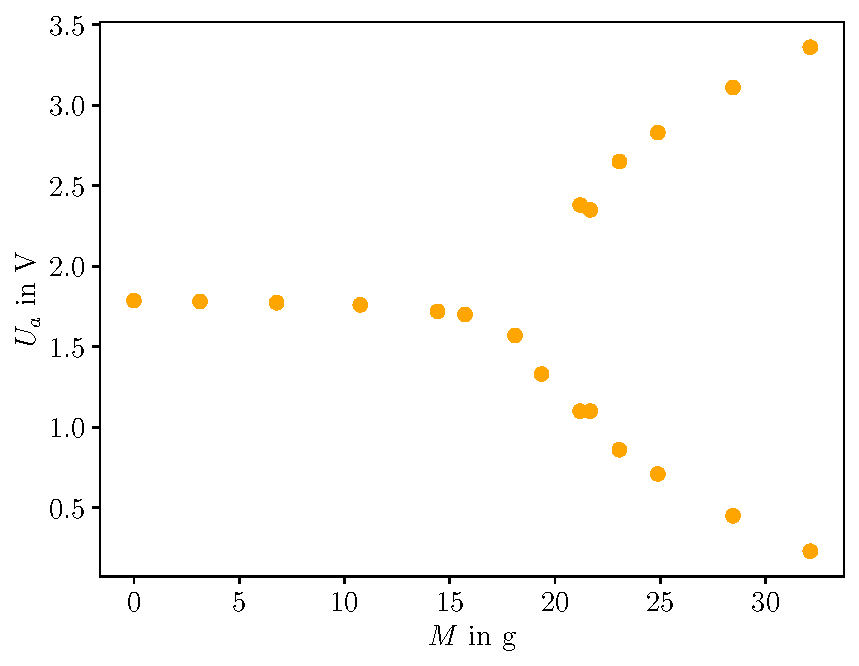
\includegraphics[scale=0.8]{Pendel/3.1/BifurkationMass.pdf}
    \captionof{figure}{Bifurkationsdiagramm in Abhängigkeit der Masse}
    \label{image:bifu}
\end{center}
Um die kritische Masse $M_k$ zu bestimmen, wird die Differenz $\Delta U_a=U_{a,l}-U_{a,r}$ bestimmt und diese quadriert, also $(\Delta U_a)^2$. Der Fehler ergibt sich dann aus dem Fehlerfortpflanzungsgesetz, wobei der Ablesefehler $s_a$ gleichzeitig als Restfehler $s_r$ abgeschätzt wird. Daraus folgt:
\begin{gather}
    (\Delta U_a)^2 = (U_{a,l}-U_{a,r})^2\\
    s_{U_a}=\sqrt{s_a^2+s_r^2}=\sqrt{2}s_a\\[0,5cm]
    s_{(\Delta U_a)^2}=\sqrt{\left(\frac{\partial((\Delta U_a)^2)}{\partial U_{a,l}}s_{U_a}\right)^2 + \left(\frac{\partial((\Delta U_a)^2)}{\partial U_{a,r}}s_{U_a}\right)^2}=2\sqrt{2}s_{U_a}|\Delta U_a|=4s_a |\Delta U_a|
\end{gather}
\begin{center}
    \begin{tabular}{r|cccc|cc}
        $M$/g &  $U_{a,l}$/V &  $U_{a,r}$/V & $s_a$/V & s_{U_a}/V & $(\Delta U_a)^2$/V$^2$ &  $s_{(\Delta U_a)^2}$/V$^2$ \\
        \hline
         0,00  &  1,78606 &  1,78606 &   0,00005 &  0,00007 &  0,0 &     0,0 \\
         3,14  &  1,78046 &  1,78046 &   0,00050 &  0,00071 &  0,0 &     0,0 \\
         6,78  &  1,77300 &  1,77300 &   0,00500 &  0,00707 &  0,0 &     0,0 \\
        10,75  &  1,76000 &  1,76000 &   0,00500 &  0,00707 &  0,0 &     0,0 \\
        14,42  &  1,72000 &  1,72000 &   0,05000 &  0,07071 &  0,0 &     0,0 \\
        15,72  &  1,70000 &  1,70000 &   0,05000 &  0,07071 &  0,0 &     0,0 \\
        18,10  &  1,57000 &  1,57000 &   0,05000 &  0,07071 &  0,0 &     0,0 \\
        19,36  &  1,33000 &  1,33000 &   0,05000 &  0,07071 &  0,0 &     0,0 \\
        21,19  &  1,10000 &  2,38000 &   0,05000 &  0,07071 &  1,6 &     0,3 \\
        21,67  &  1,10000 &  2,35000 &   0,05000 &  0,07071 &  1,6 &     0,3 \\
        23,05  &  0,86000 &  2,65000 &   0,05000 &  0,07071 &  3,2 &     0,4 \\
        24,88  &  0,71000 &  2,83000 &   0,05000 &  0,07071 &  4,5 &     0,4 \\
        28,45  &  0,45000 &  3,11000 &   0,05000 &  0,07071 &  7,1 &     0,5 \\
        32,12  &  0,23000 &  3,36000 &   0,05000 &  0,07071 &  9,8 &     0,6 \\
    \end{tabular}
    \captionof{table}{Messreihe Auslenkung Gleichgewichtslage}
    \label{tab:gleichgewichtslage}
\end{center}
Die Daten werden dann mit dem Numpy-Modul linear gefittet, dabei werden nur die letzten sieben Datensätze verwendet werden, da sich $(\Delta U_a)^2$ erst ab da Veränderung zeigt (siehe Abb. \ref{image:linFit}). Dabei ergibt sich die gefittete Funktion mit den jeweiligen Fehlern:
\begin{gather}
    (\Delta U_a)^2 = c M + b = 0,77 \frac{\text{V}^2}{\text{g}} M - 14,73~\text{V}^2\\
    c = (0,77 \pm 0,02)~\frac{\text{V}^2}{\text{g}},~b = (-14,73 \pm 0,48)~\text{V}^2
\end{gather}
Daraus ergibt sich die kritische Masse $M_k$, wenn man $(\Delta U_a)^2=0$ setzt. Woraus widerrum mit Fehlerfortpflanzung folgt:
\begin{gather}
    M_k = \frac{b}{c} = 19,22~\text {g},~
    s_{M_k} = \sqrt{\left(\frac{s_b}{c}\right)^2+\left(\frac{b s_c}{c^2}\right)^2}=0,78~\text{g}\\[0,5cm]
    \Rightarrow\boxed{M_k = (19,22 \pm 0,78)~\text{g}}
\end{gather}
Die Federkonstante $k$ und dessen Fehler ergibt sich dann mit dem Fehler der Länge $L$ (gemessen mit Stahlmaßstab), wobei die Erdbeschleunigung fehlerfrei angenommen wird:
\begin{gather}
    L = 0,37~\text{m}\\
    s_L=\sqrt{s_a^2+s_r^2}=\sqrt{(5\cdot 10^{-4}~\text{m})^2+(5\cdot 10^{-5}~\text{m}+\cdot 10^{-4}*L)^2} = 0,0006~\text{m}\\
    M_k = \frac{k}{gL} \Leftrightarrow k = M_k g L = 0,069762834~\text{Nm}\\
    s_k = \sqrt{(gLs_{M_k})^2+(M_kgs_L)^2} = 0,002833425~\text{Nm}\\[0,5cm]
    \Rightarrow\boxed{k = (0,070 \pm 0,003)~\text{Nm}}
\end{gather}
Hierbei ist anzumerken, dass $k$ nicht die Einheit einer Federkonstante hat sondern eines Drehmoments. Die Vermutung liegt mit einen Blick auf Kapitel \ref{sub:bewegungsgleichung} beschrieben Differentialgleichung, dass sich bei $k$ eigentlich um das Direktionsmoment handeln muss, wobei das Direktionsmoment der Federkonstante $k$ bei longitudinalen Auslenkungen entspricht.

Zur Verifikation des Ergebnisses haben wir mehrfache (10mal) die Schwingungsdauer des Pendels mit der befestigten Masse $M = 12,58$ g gemessen.
\begin{center}
    \begin{tabular}{ c | cccccccccc }
        {} & 1 & 2 & 3 &4 &5 &6 &7 &8 &9 &10\\
        \hline
        $T_10$/s&19,14&19,28&18,88&19,18&19,00&18,66&19,12&19,01&19,20&19,29\\
    \end{tabular}
    \captionof{table}{Messreihe Schwingungsdauer}
    \label{tab:schwingung}
\end{center}
Es wird nun der Mittelwert über eine Periode genommen, wobei der Ablesefehler der digitale Messuhr auch gleichzeitig als Restfehler abgeschätzt wird und der Fehler der einen Periode mit dem Fehlerfortpflanzungsgesetz berechnet wurde. Daraus folgt:
\begin{gather}
    T = \overline{T} = \frac{1}{10} \sum_{n = 1}^{10} \frac{T_{10,n}}{10} = 1,9076~\text{s}\\
    s_{T_{10}} = \sqrt{s_a^2+s_r^2}=\sqrt{2}s_a \Rightarrow s_T = \frac{s_T}{10\sqrt{10}} = \frac{s_a}{10\sqrt{5}} = 0,000447214\\[0,5cm]
    \Rightarrow\boxed{T = (1,9076 \pm 0,0004)~\text{s}}
\end{gather}
\newpage
Über Federkonstante (Direktionsmoment) $k$ lässt sich dann die Schwingungsdauer $T$ wie folgt berechnen \citep{Leifi}, wobei für den Fehler von $T$ der Fehler der Masse und Länge vernachlässigt wird:
\begin{gather}
    T = 2\pi\sqrt{\frac{ML^2}{k- MgL}} = 1,671383586~\text{s}\\
    s_T = \frac{\pi ML^2 s_k}{(k-MgL)^2 \sqrt{\frac{ML^2}{k- MgL}}} = 0,1030091566\\[0,5cm]
    \Rightarrow\boxed{T = (1,67 \pm 0,10)~\text{s}}
\end{gather}
Das Ergebnis zeigt, dass die bestimmte Federkonstante $k$ nahe an den tatsächlichen Wert der Blattfeder liegt. Die möglichen Abweichung könnten von denen in Kapitel \ref{sub:bewegungsgleichung} gemachten Näherungen oder dem vorangegangenen Fit verursacht werden. Auch könnte das Alter des Messaufbaus seinen Teil zu der Ungenauigkeit beigetragen haben. Dennoch ist das Ergebnis im Rahmen unserer Möglichkeiten akzeptabel.
\newpage
\begin{center}
    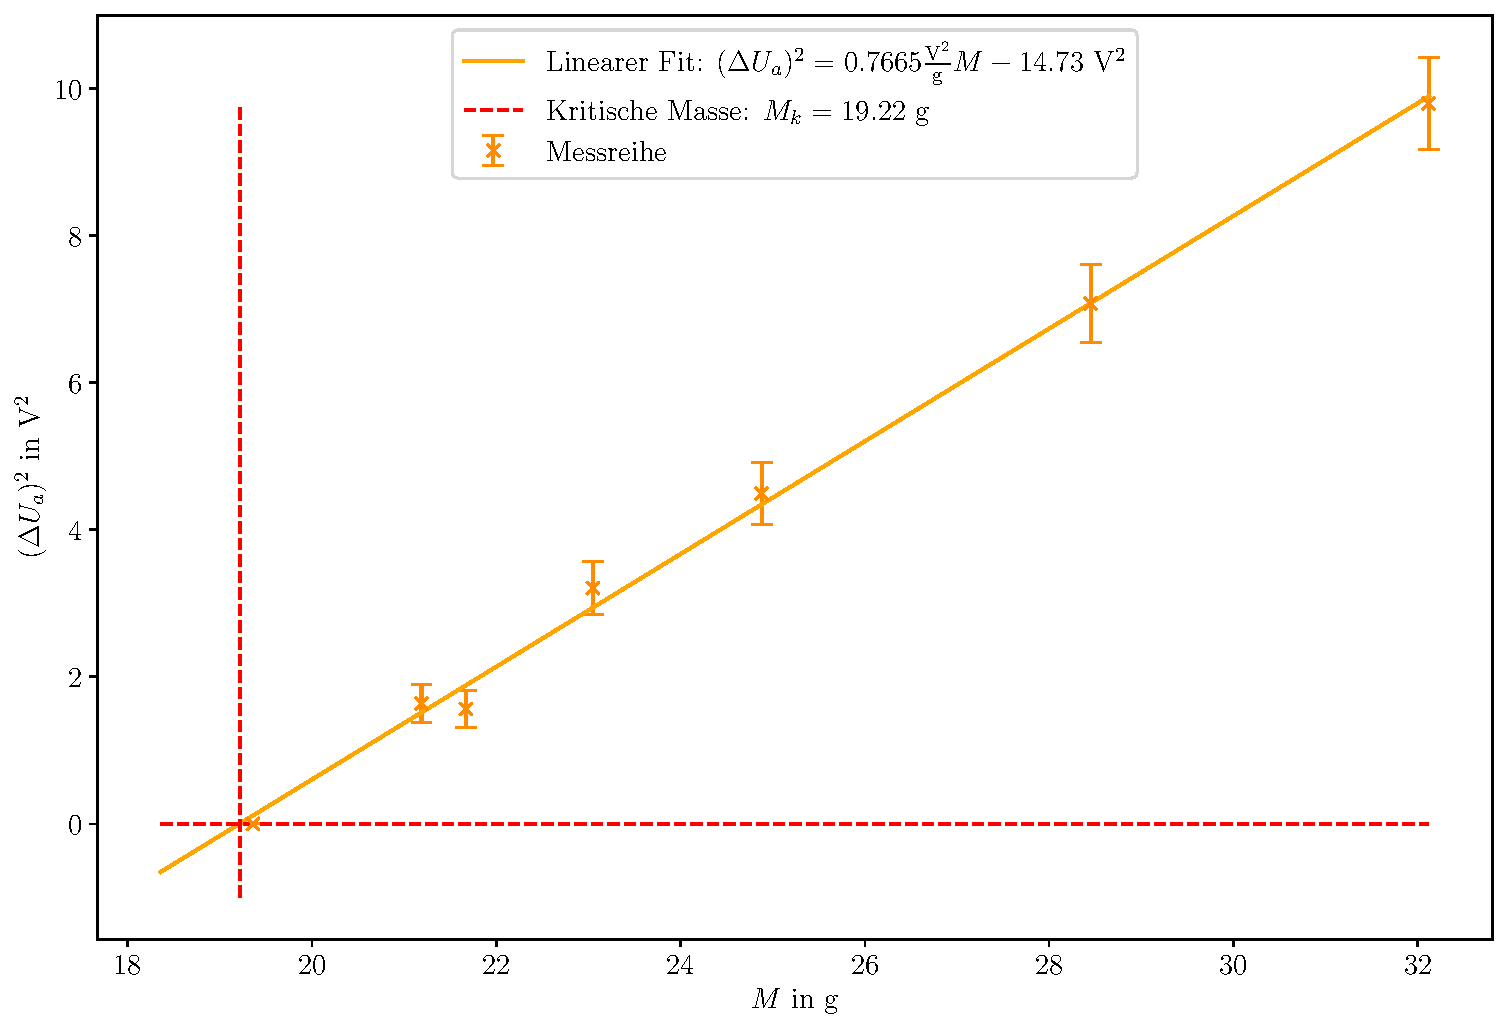
\includegraphics[scale=0.75, angle=90]{Pendel/3.1/linearFit.pdf}
    \captionof{figure}{Linerar Fit der Messreihe}
    \label{image:linFit}
\end{center}

\subsection{Schwache Nichtlinearität}
\label{sub:AuswertungweakLin}
\paragraph{a)} \textbf{Amplitudenabhängigkeit}\\
Für die experimentelle Auswertung der Amplitudenabhängigkeit der Schwingungsdauer $T$ des Pendels  werden aus den aufgenommenen Daten die Maxima der Spannung $U_{a}$ bestimmt, sowie der zeitlichen Abstand $\Delta t$ zwischen zwei Maxima ermittelt. Der Abstand $\Delta t$ entspricht dann der Periodendauer $T$ des Pendels. Da mehrere Werte für $T$ gehäuft vorkamen, haben wir die Daten von $T$ gruppiert und über die zugehörigen Maxima der Spannung $U_{a,max}$ den Mittelwert gebildet.
\begin{center}
    \begin{tabular}{l|c c c c c c c c}
        $T$/s & 1.90 & 2.10 & 2.20 & 2.30 & 2.32 & 2.36 & 2.40 & 2.44\\
        \hline
        $U_{a,max}$/V &  2.3950  &  2.2310  &  2.0450  &  1.8816  &  1.7230  &  1.5400  &  1.6278  &  1.5651 \\
        \end{tabular}
        \captionof{table}{Messreihe Schwingungsdauer in Amplitudenabhängigkeit}
\end{center}
\begin{center}
    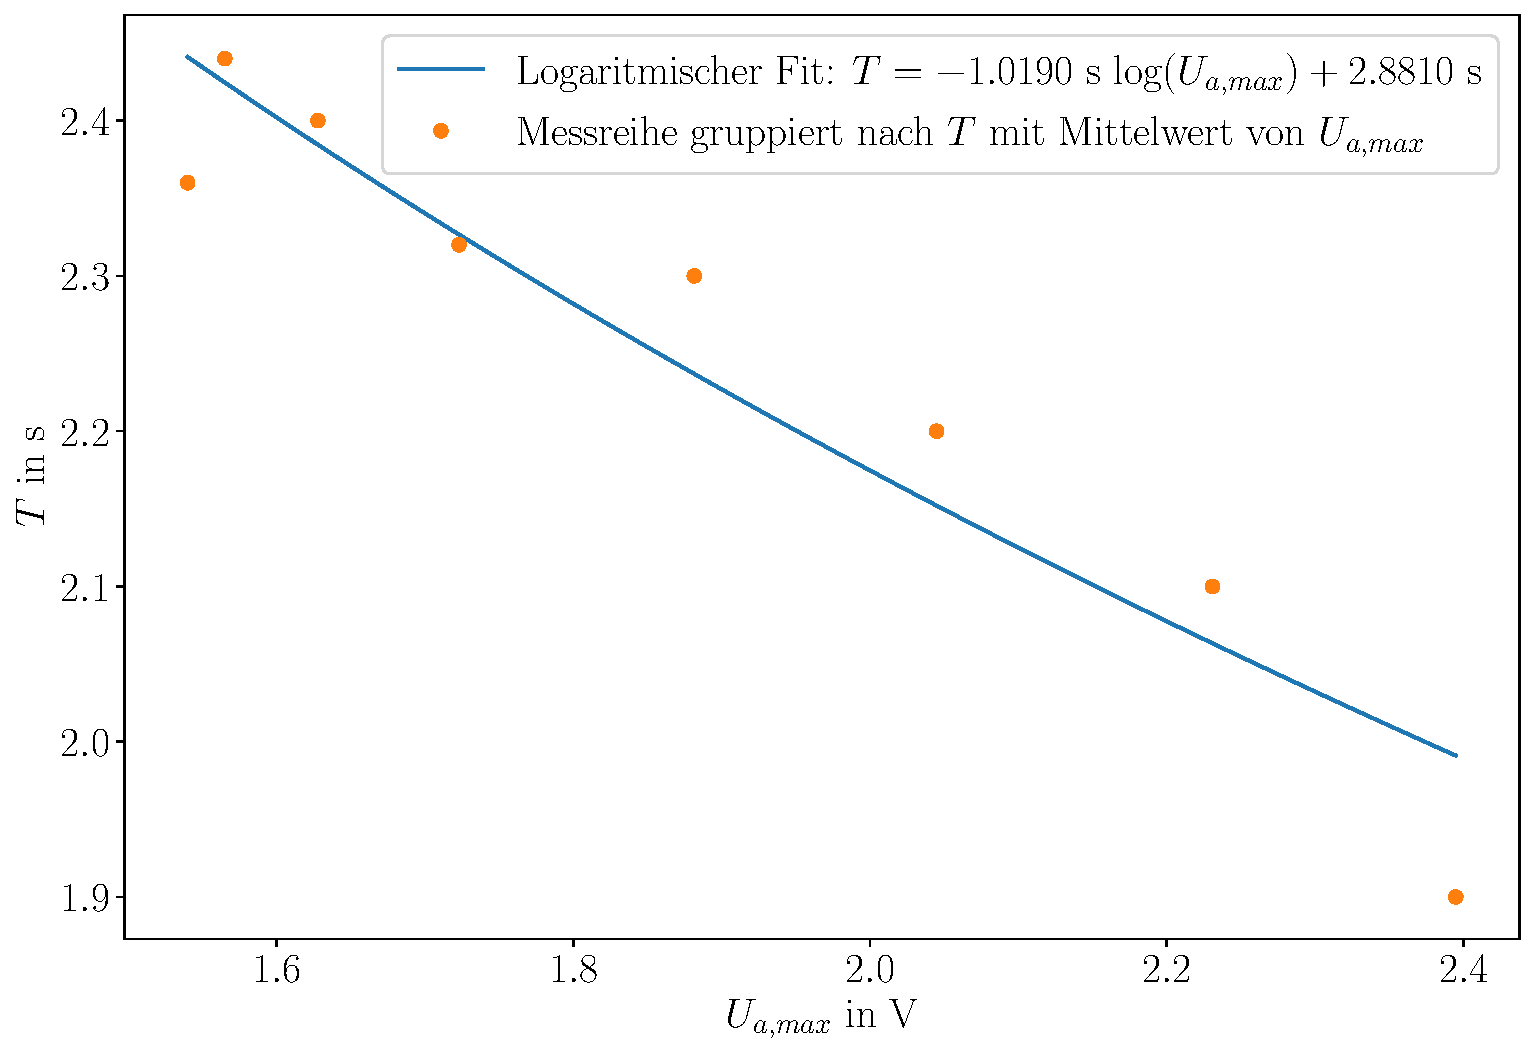
\includegraphics[scale=0.5]{Pendel/3.2a/AbhSchwingung.pdf}
    \captionof{figure}{Ampliudenabhängigkeit der Schwingungsdauer mit logarithmischen Fit}
    \label{image:schwing}
\end{center}
Bei der grafischen Auswertung (siehe Abb.\ref{image:schwing}) erkennt man deutlich einen Abwärtstrend. Ein logarithmischer Fit wie in Kapitel \ref{sub:schwingungsdauer} beschrieben, gibt dann die Funktion:
\begin{gather}
    T=(-1,0190~\text{s})\log(U_{a,max}) + (2.8810~\text{s}).
\end{gather}
Dieser Fit ist aber noch nicht aussagekräftig, da die Messwerte auch einen linearen Fit zulassen würden, weswegen mehr Messpunkte gebraucht werden würden.
\paragraph{b)} \textbf{Resonanzkurve}\\
Bei der Messung der Resonanzkurve erkennt man grob verschiedene Bereiche (siehe Abb \ref{image:resonanz}), dabei beschreibt die \textcolor{blue}{blaue Kurve} den Hinweg (\SI{0,0}{\hertz}$\rightarrow$\SI{6,9}{\hertz}) und die \textcolor{orange}{orange Kurve} den Rückweg (\SI{6,9}{\hertz} $\rightarrow$ \SI{0,0}{\hertz}).\\

Zuerst betrachten wir den Hinweg bzw. die \textcolor{blue}{blaue Kurve}:
\begin{itemize}
    \item[1)]0,0-0,5 Hz\\Die Drehfrequenz des Schrittmotors reicht nicht aus um das Pendel anzuregen.
    \item[2)]0,5-2,0 Hz\\Erregerfrequenz regt Pendel zur Schwingung an. Vereinzelte Zacken zeigen dabei die Schritte, welche der Schrittmotor macht beim Antreiben.
    \item[3)]2,0-4,0 Hz\\Anstieg der Amplitude bis zu ihrem Maximum von $\approx\SI{2,2}{\volt}$
    \item[5)]4,0-6,9 Hz\\Abfallen der Amplitude bis auf \SI{0}{\hertz}, wobei das Pendel der Drehfrequenz des Motors nicht nachkommt.\\
\end{itemize}

Nun betrachten wir den Rückweg bzw. die \textcolor{orange}{orange Kurve}:
\begin{itemize}
    \item[1)]6,9-3,0 Hz\\Anstieg der Amplitude von \SI{0}{\hertz} auf ihr Maximum von $\approx\SI{2,0}{\volt}$.
    \item[2)]3,0-2,0 Hz\\Abfallen der Amplitude auf $\approx\SI{0,6}{\volt}$ 
    \item[3)]2,0-0,5 Hz\\Erregerfrequenz regt Pendel zur Schwingung an. Vereinzelte Zacken zeigen dabei die Schritte, welche der Schrittmotor macht beim Antreiben.
    \item[5)]0,5-0,0 Hz\\Die Drehfrequenz des Schrittmotors reicht nicht aus um das Pendel anzuregen.\\
\end{itemize}
Im Bereich zwischen \SI{3,0}{\hertz} und \SI{4,0}{\hertz} lässt sich dann durch Vergleich zwischen Hin- und Rückweg schön den bistabilen Zustand aus Kapitel \ref{sub:schwingungsdauer}.
\newpage
\begin{center}
    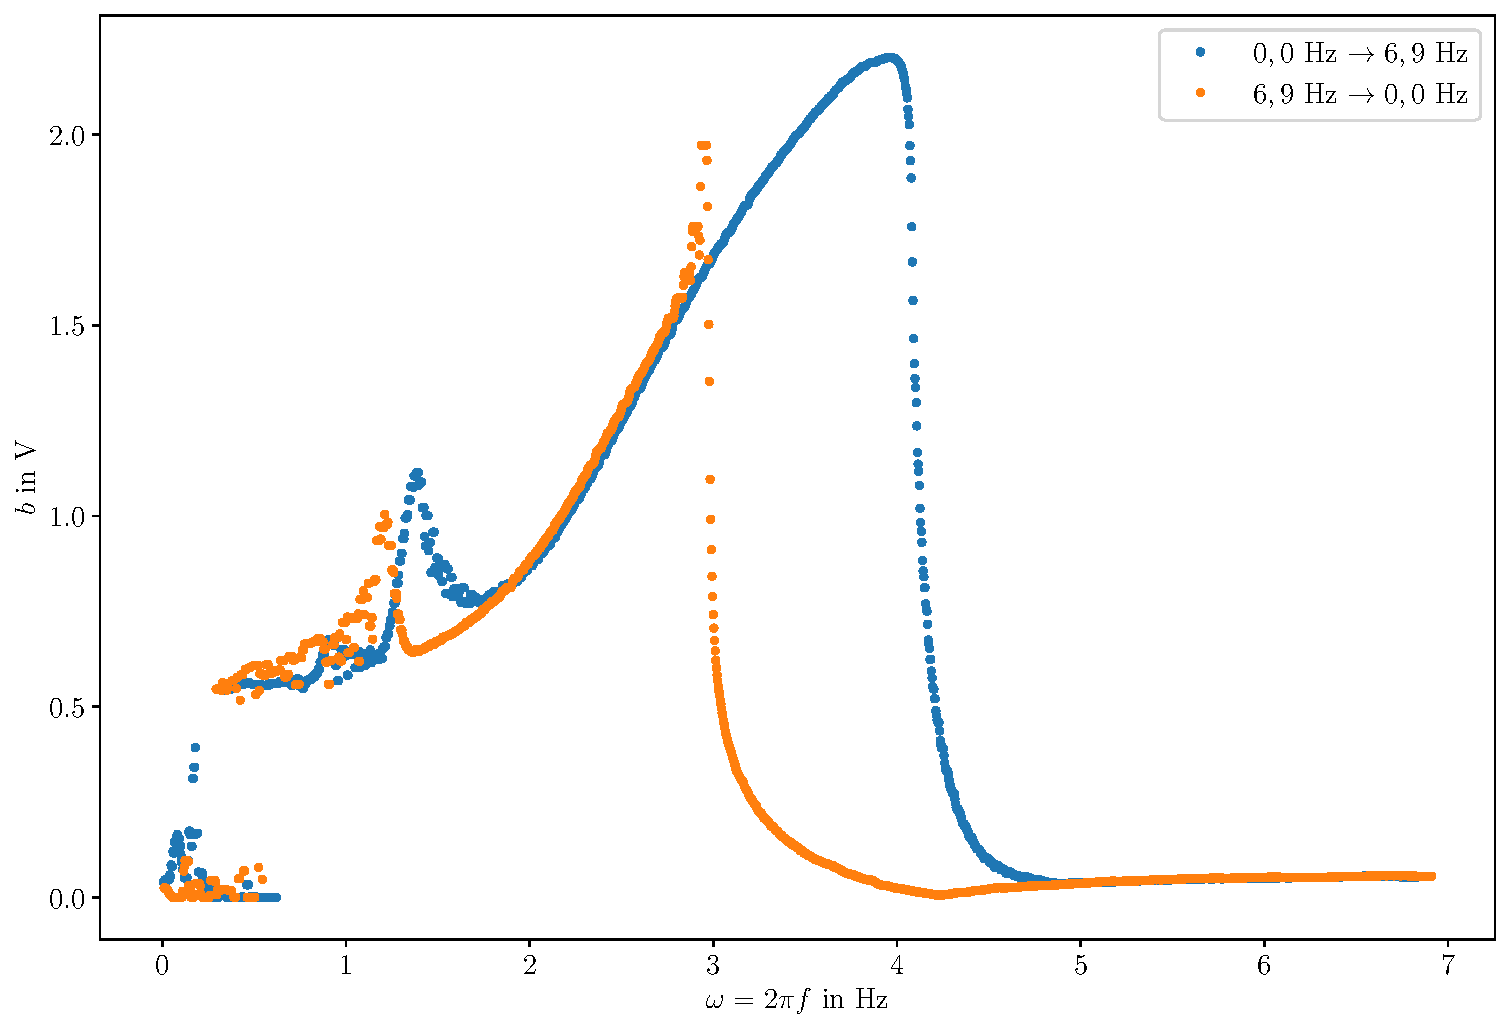
\includegraphics[scale=0.75, angle=90]{Pendel/3.2b/Resonanz.pdf}
    \captionof{figure}{Resonanzkurve}
    \label{image:resonanz}
\end{center}
\newpage

\subsection{Starke Nichtlinearität}
\label{sub:AuswertungstrongLin}
\paragraph{a)} \textbf{Schwinungszustände des Pendels}\\
Nun werden die einzelnen Schwingungszustände bei verschiedenen Frequenzen untersucht. Wobei mit einer hohen Frequenz begonnen wurde und dann schrittweise verkleinert wird.\\

In Abb. \ref{image:0,233hz} zeigt das Pendel chaotisches Verhalten, dabei befindet es sich selbst auf der linken Seite. Im Leistungsspektrum erkennt man aber ausgeprägte Zacken, was für ein quasi-periodisches Verhalten sprechen könnte. 
\begin{center}
    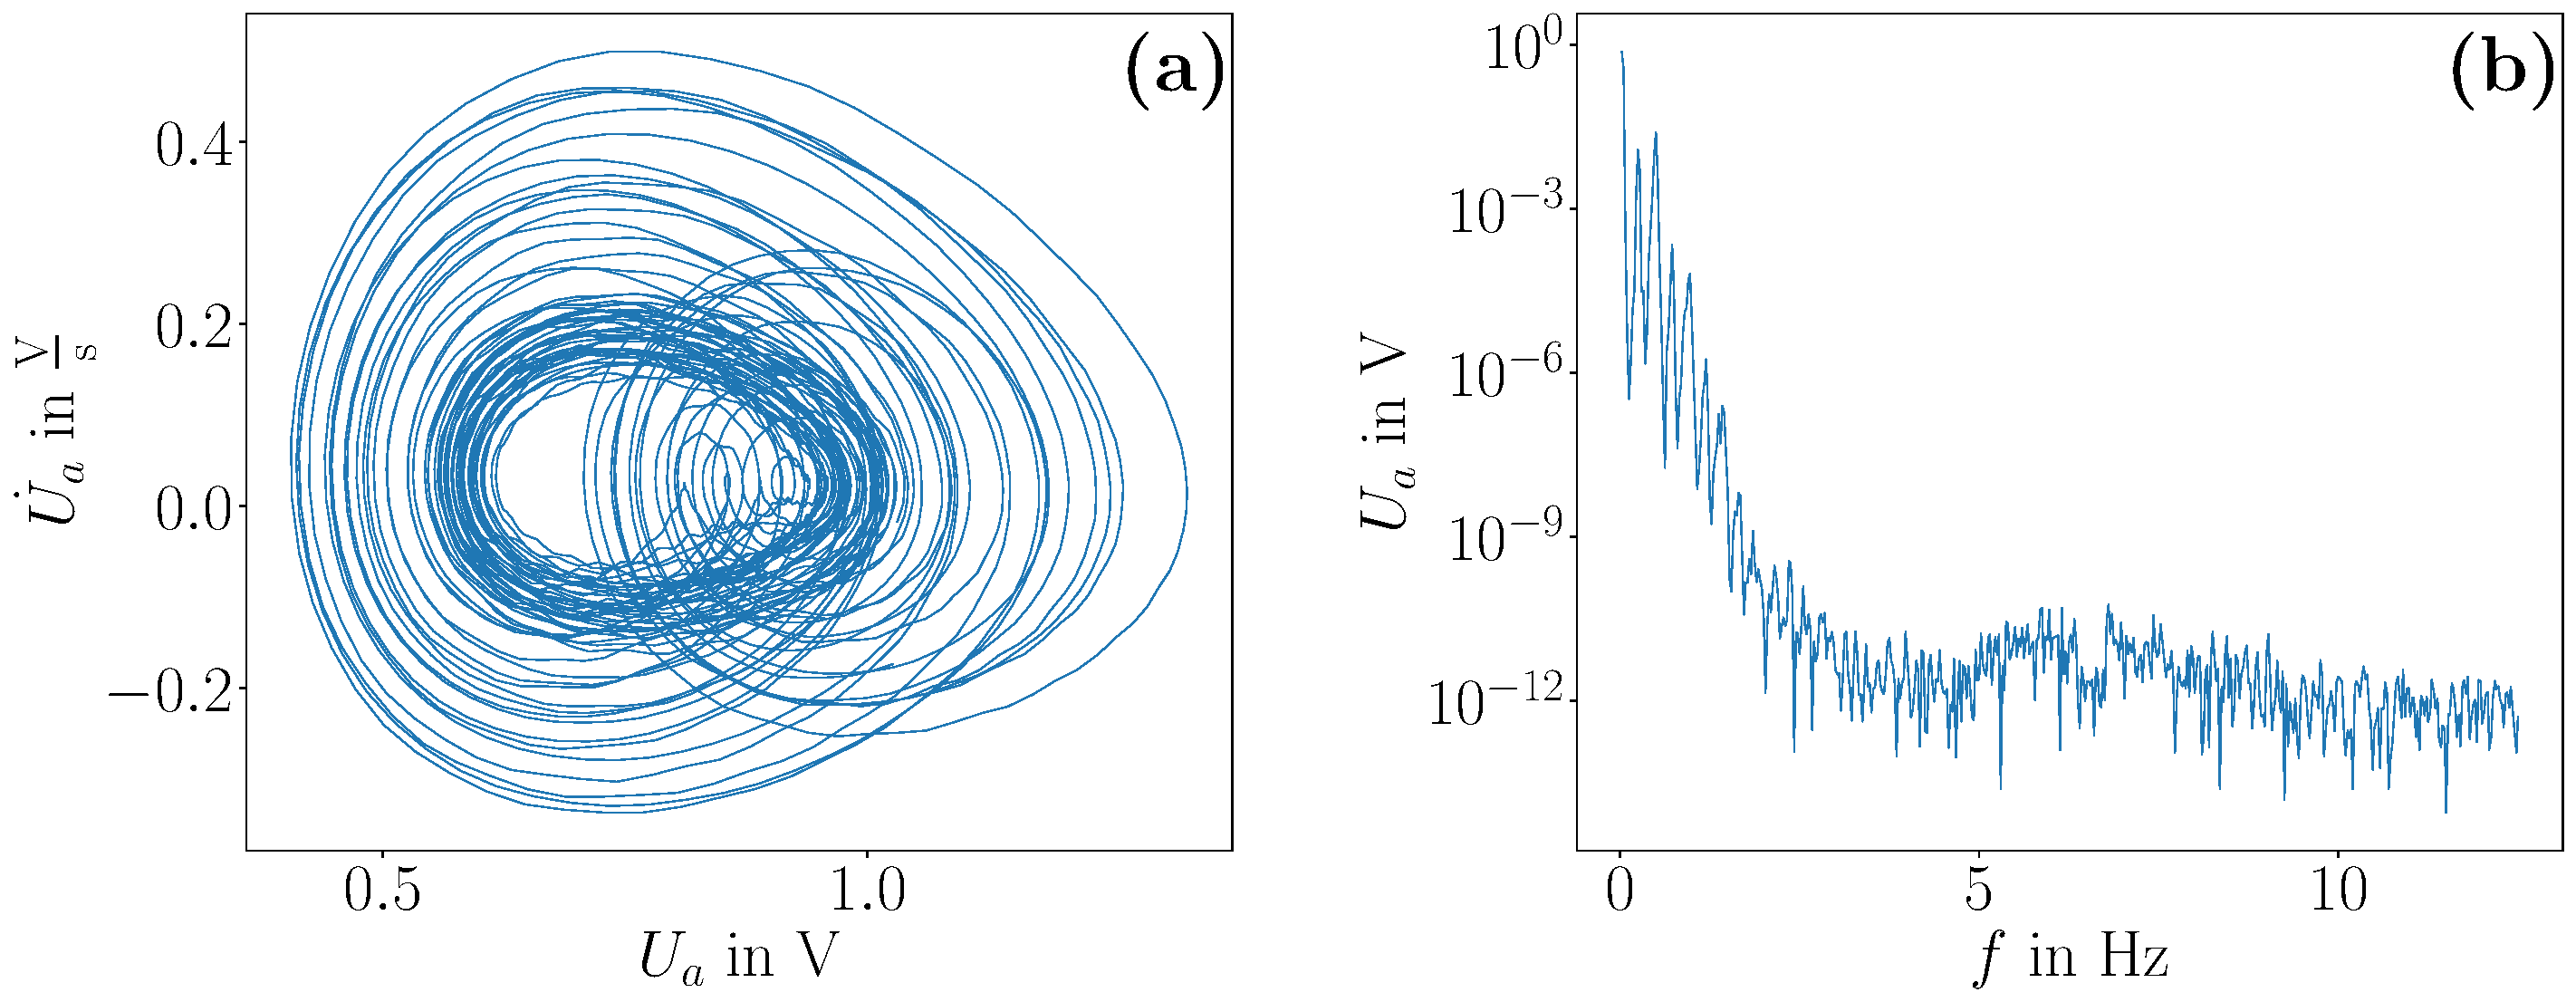
\includegraphics[scale=0.25]{Pendel/3.3a/0,233Hz.pdf}
    \captionof{figure}{Messung bei $f_a$=0,233 Hz, (a) Phasenportrait (b) Leistungsspektrum}
    \label{image:0,233hz}
\end{center}
Abb. \ref{image:0,411hz} zeigt deutlich chaotisches Verhalten des Pendels, was auch am Rauschen im Leistungsspektrum auch zu erkennen ist. Weiterhin erkennt man die zwei möglichen Schwingungen auf der rechten und linken Seite der Pendels, wobei in der Mitte der Sattelpunkt des Attraktors.
\begin{center}
    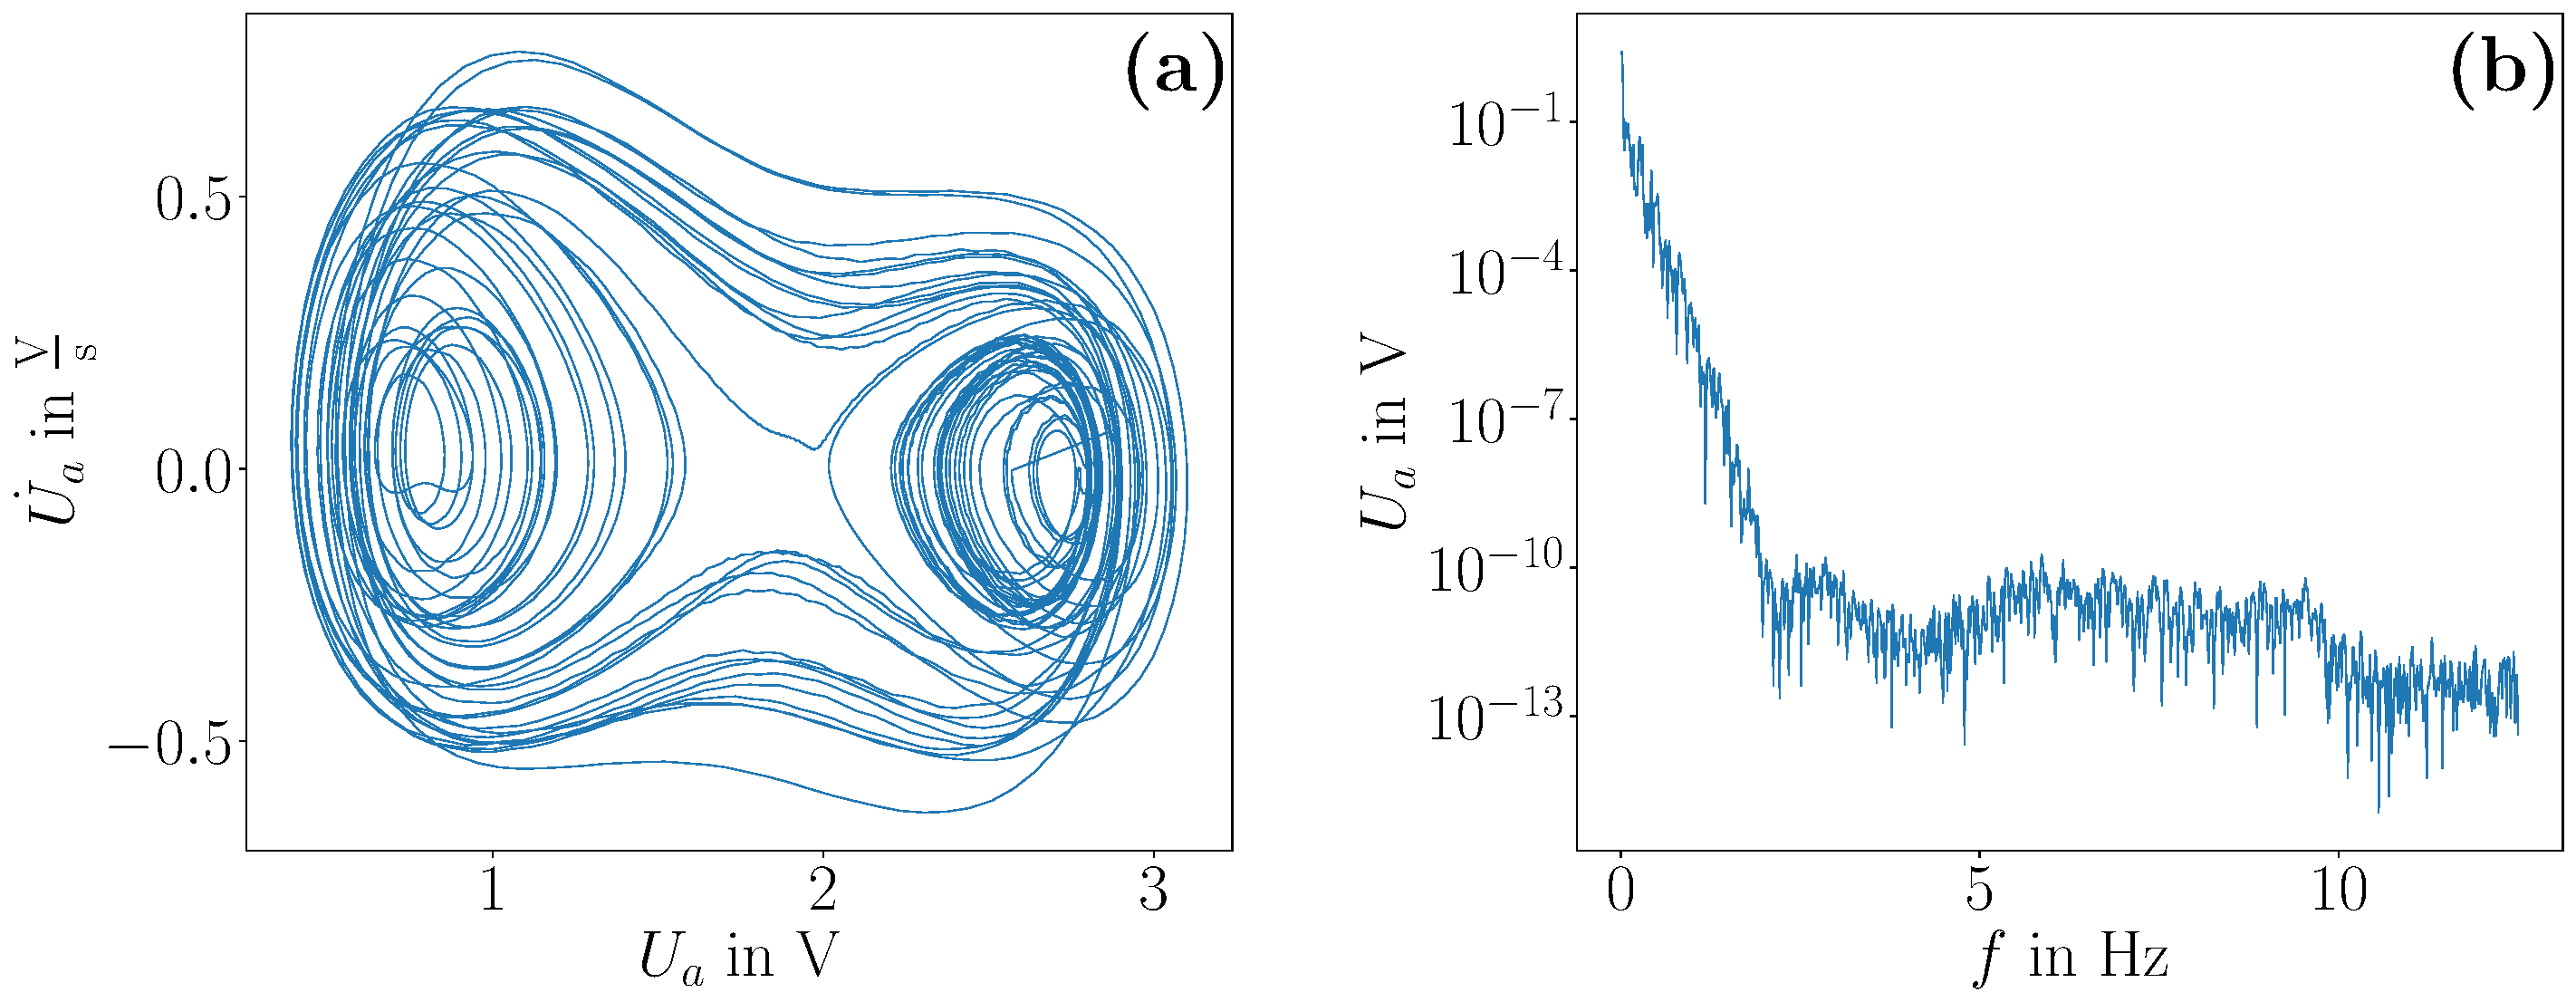
\includegraphics[scale=0.25]{Pendel/3.3a/0,411Hz.pdf}
    \captionof{figure}{Messung bei $f_a$=0,411 Hz, (a) Phasenportrait (b) Leistungsspektrum}
    \label{image:0,411hz}
\end{center}
%\begin{center}
%    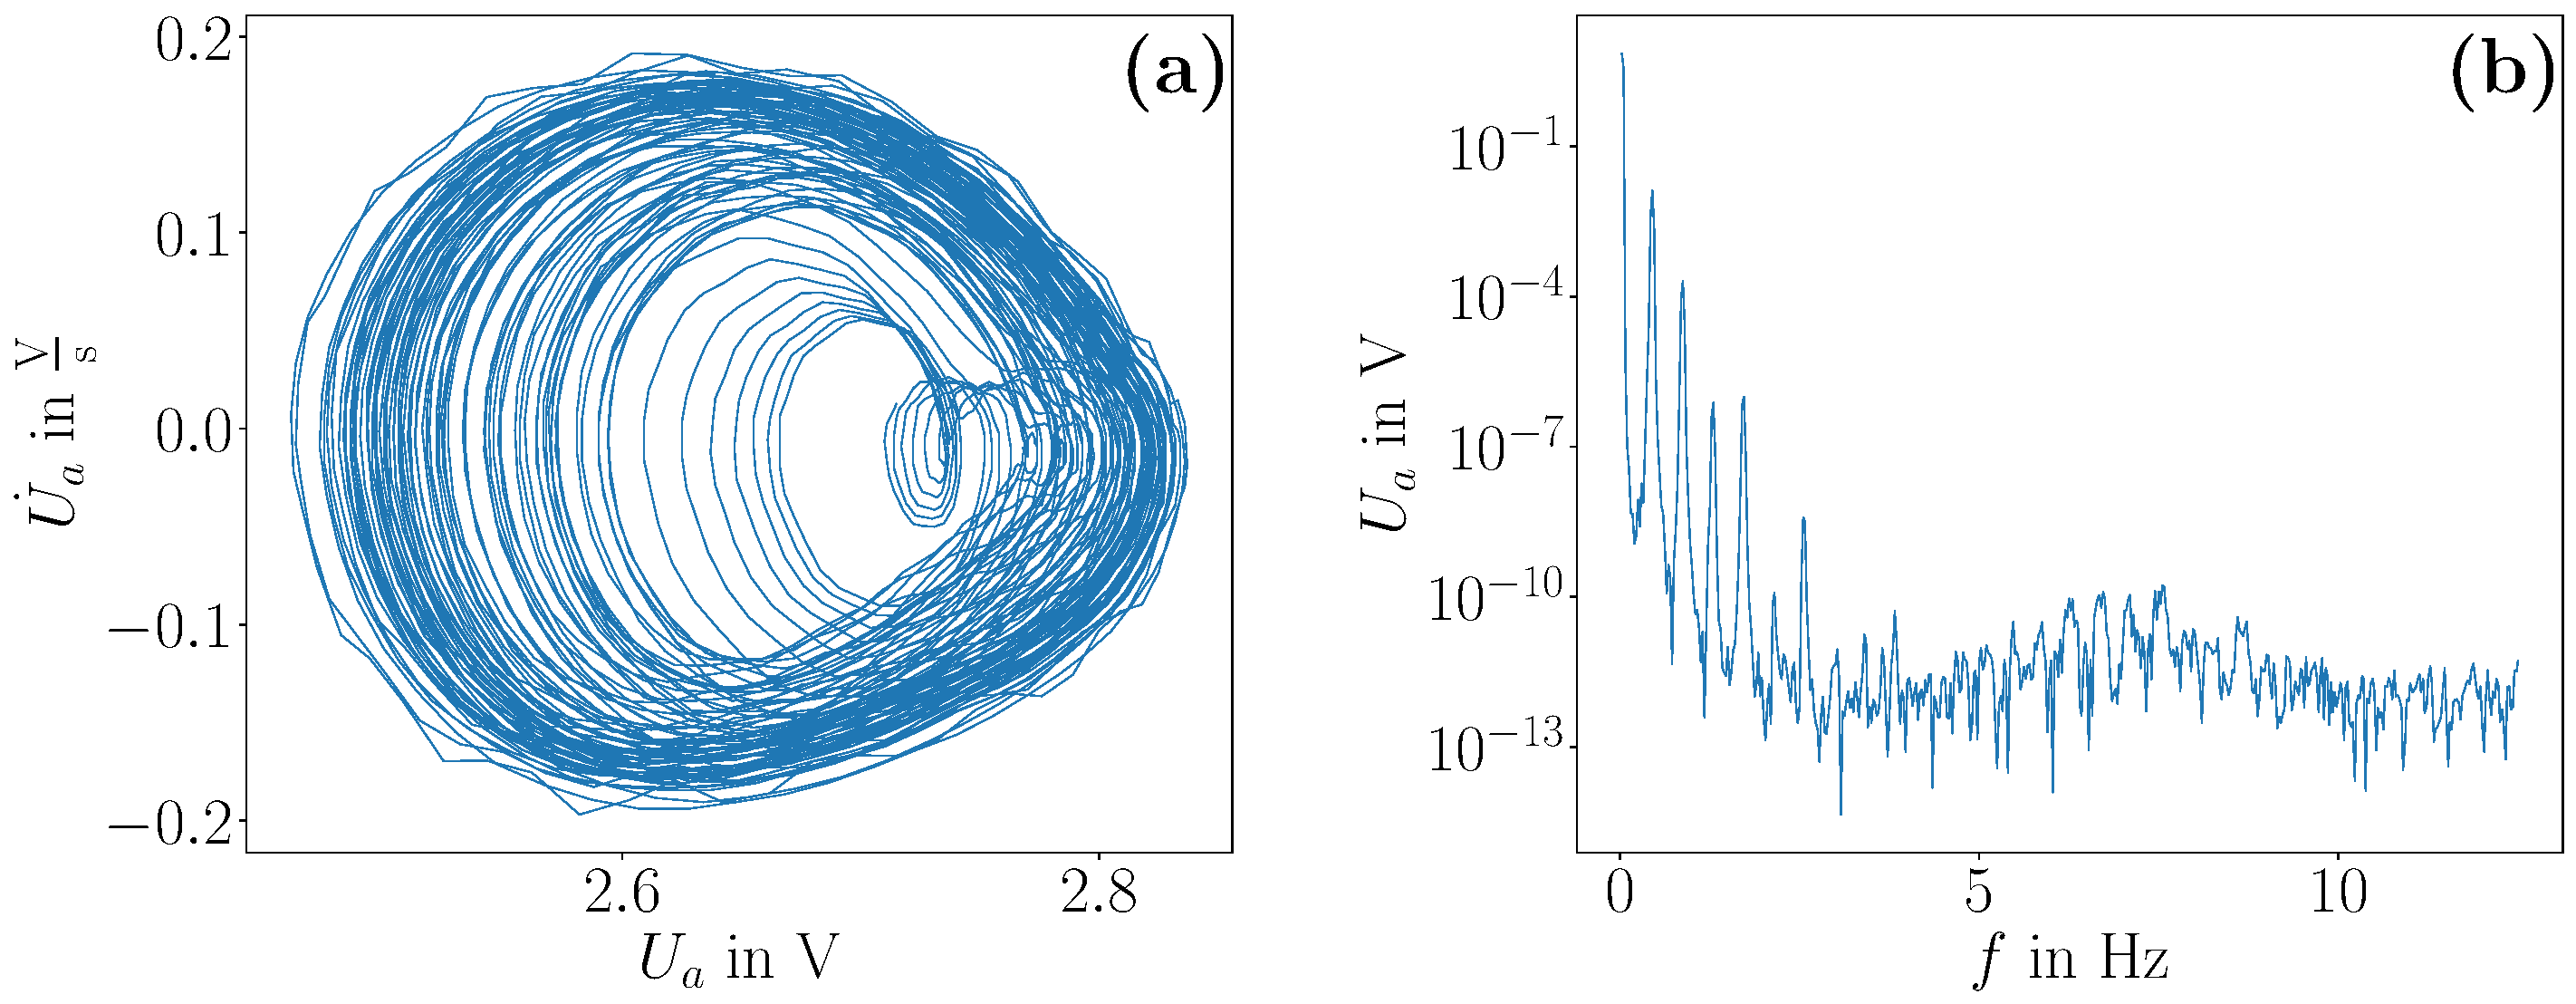
\includegraphics[scale=0.25]{Pendel/3.3a/0,847Hz.pdf}
%    \captionof{figure}{Messung bei $f_a$=0,847 Hz, (a) Phasenportrait (b) Leistungsspektrum}
%    \label{image:0,847hz}
%\end{center}
Hier erkennt man in Abb. \ref{image:0,882hz} nur ganz leicht die Periode 2 im Phasenportrait, da das Verhalten weiterhin chaotisch. Dafür sieht man im Leistungsspektrum deutliche ausgeprägte Peaks.
\begin{center}
    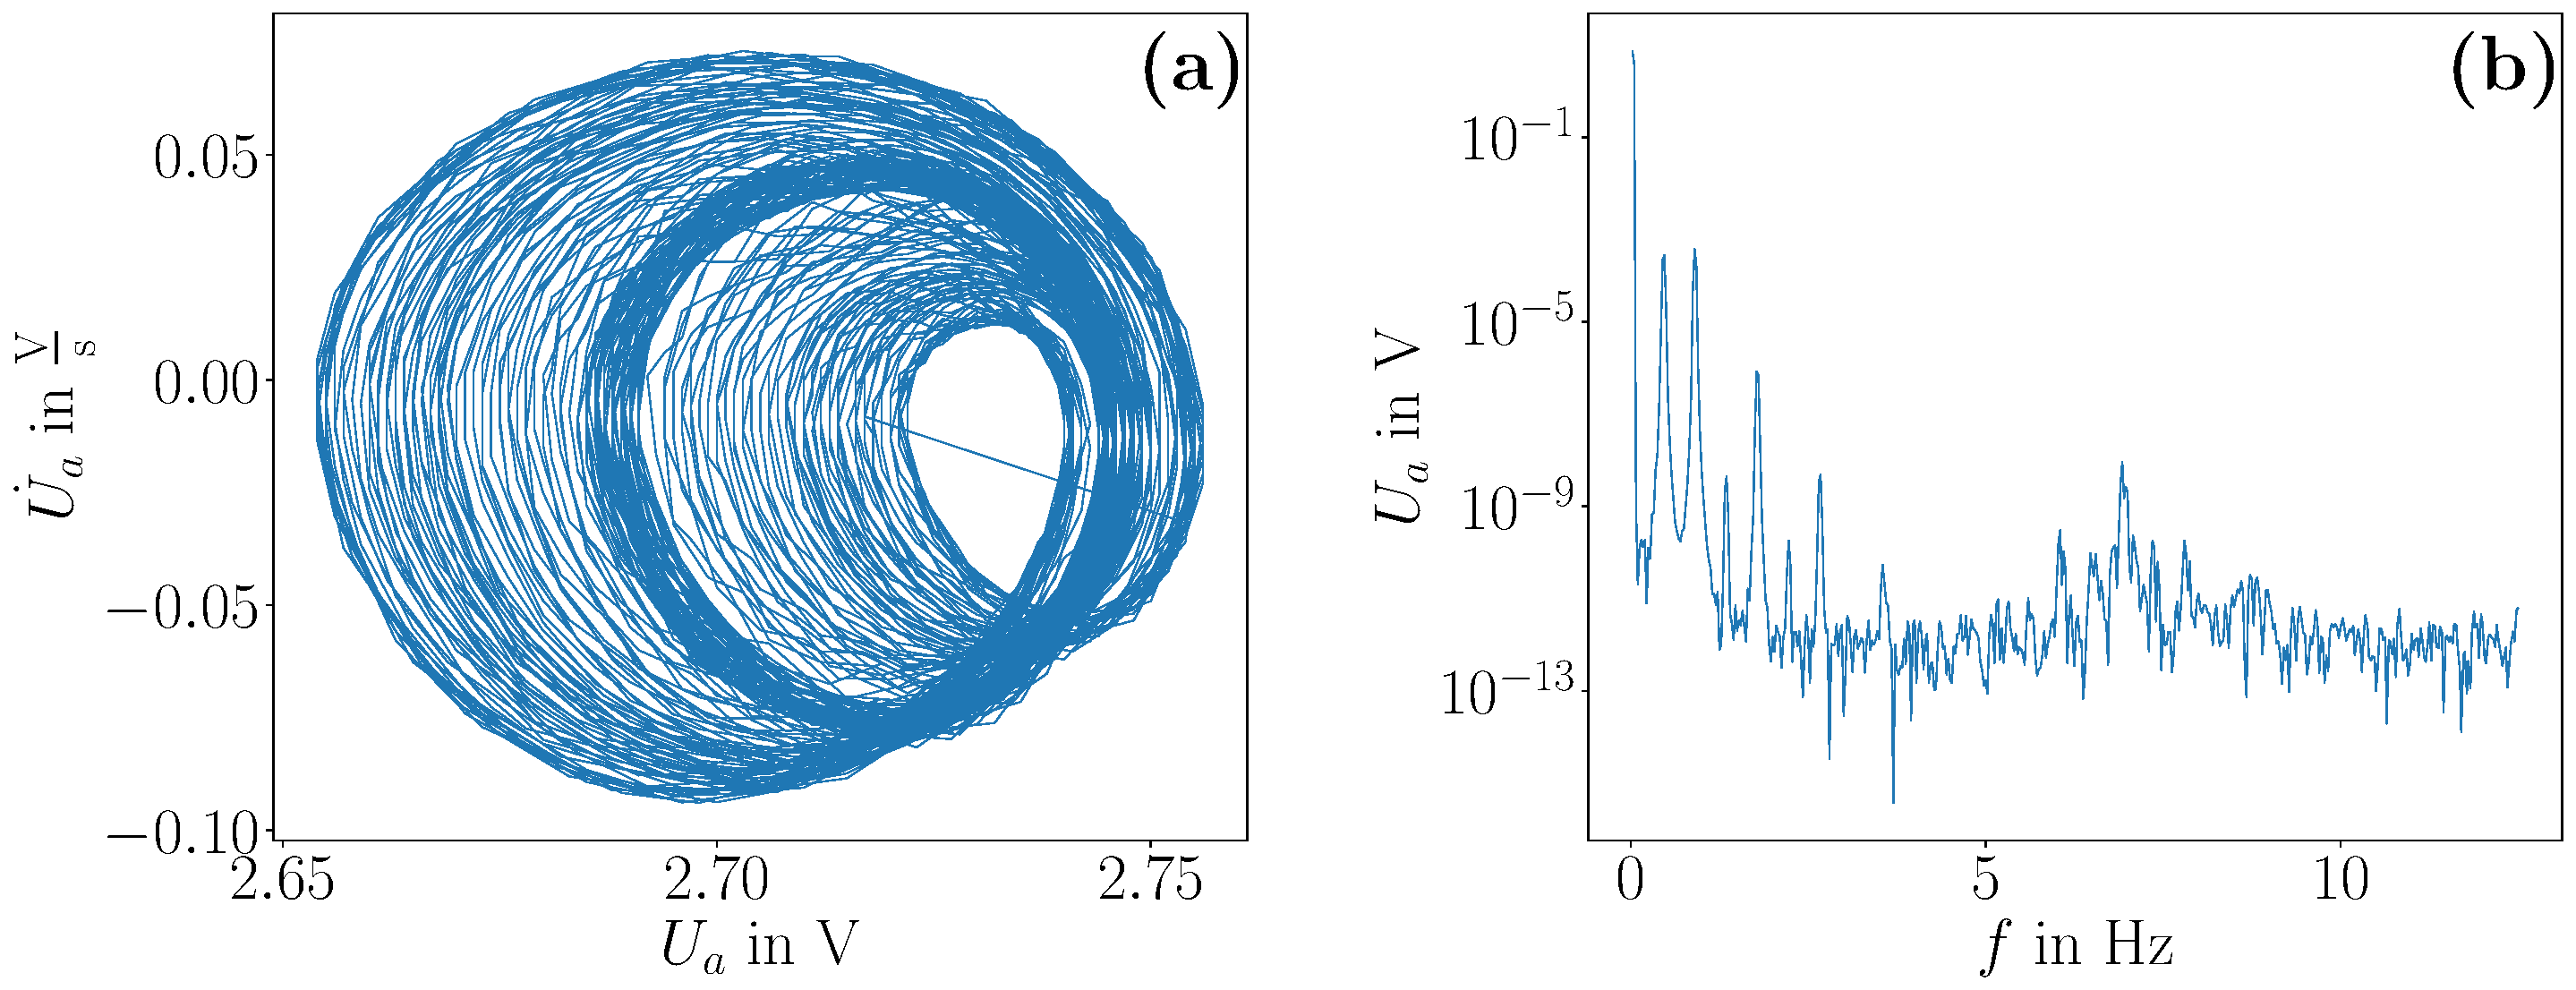
\includegraphics[scale=0.25]{Pendel/3.3a/0,882Hz.pdf}
    \captionof{figure}{Messung bei $f_a$=0,882 Hz, (a) Phasenportrait (b) Leistungsspektrum}
    \label{image:0,882hz}
\end{center}
Deutlich ausgebildete Periode 1 Schwingung in Abb. \ref{image:1,201hz}, gut zu erkennen an dem Attraktor in Form eines leicht deformierten Kreises und an den definierten Peaks im Leistungsspektrum.
\begin{center}
    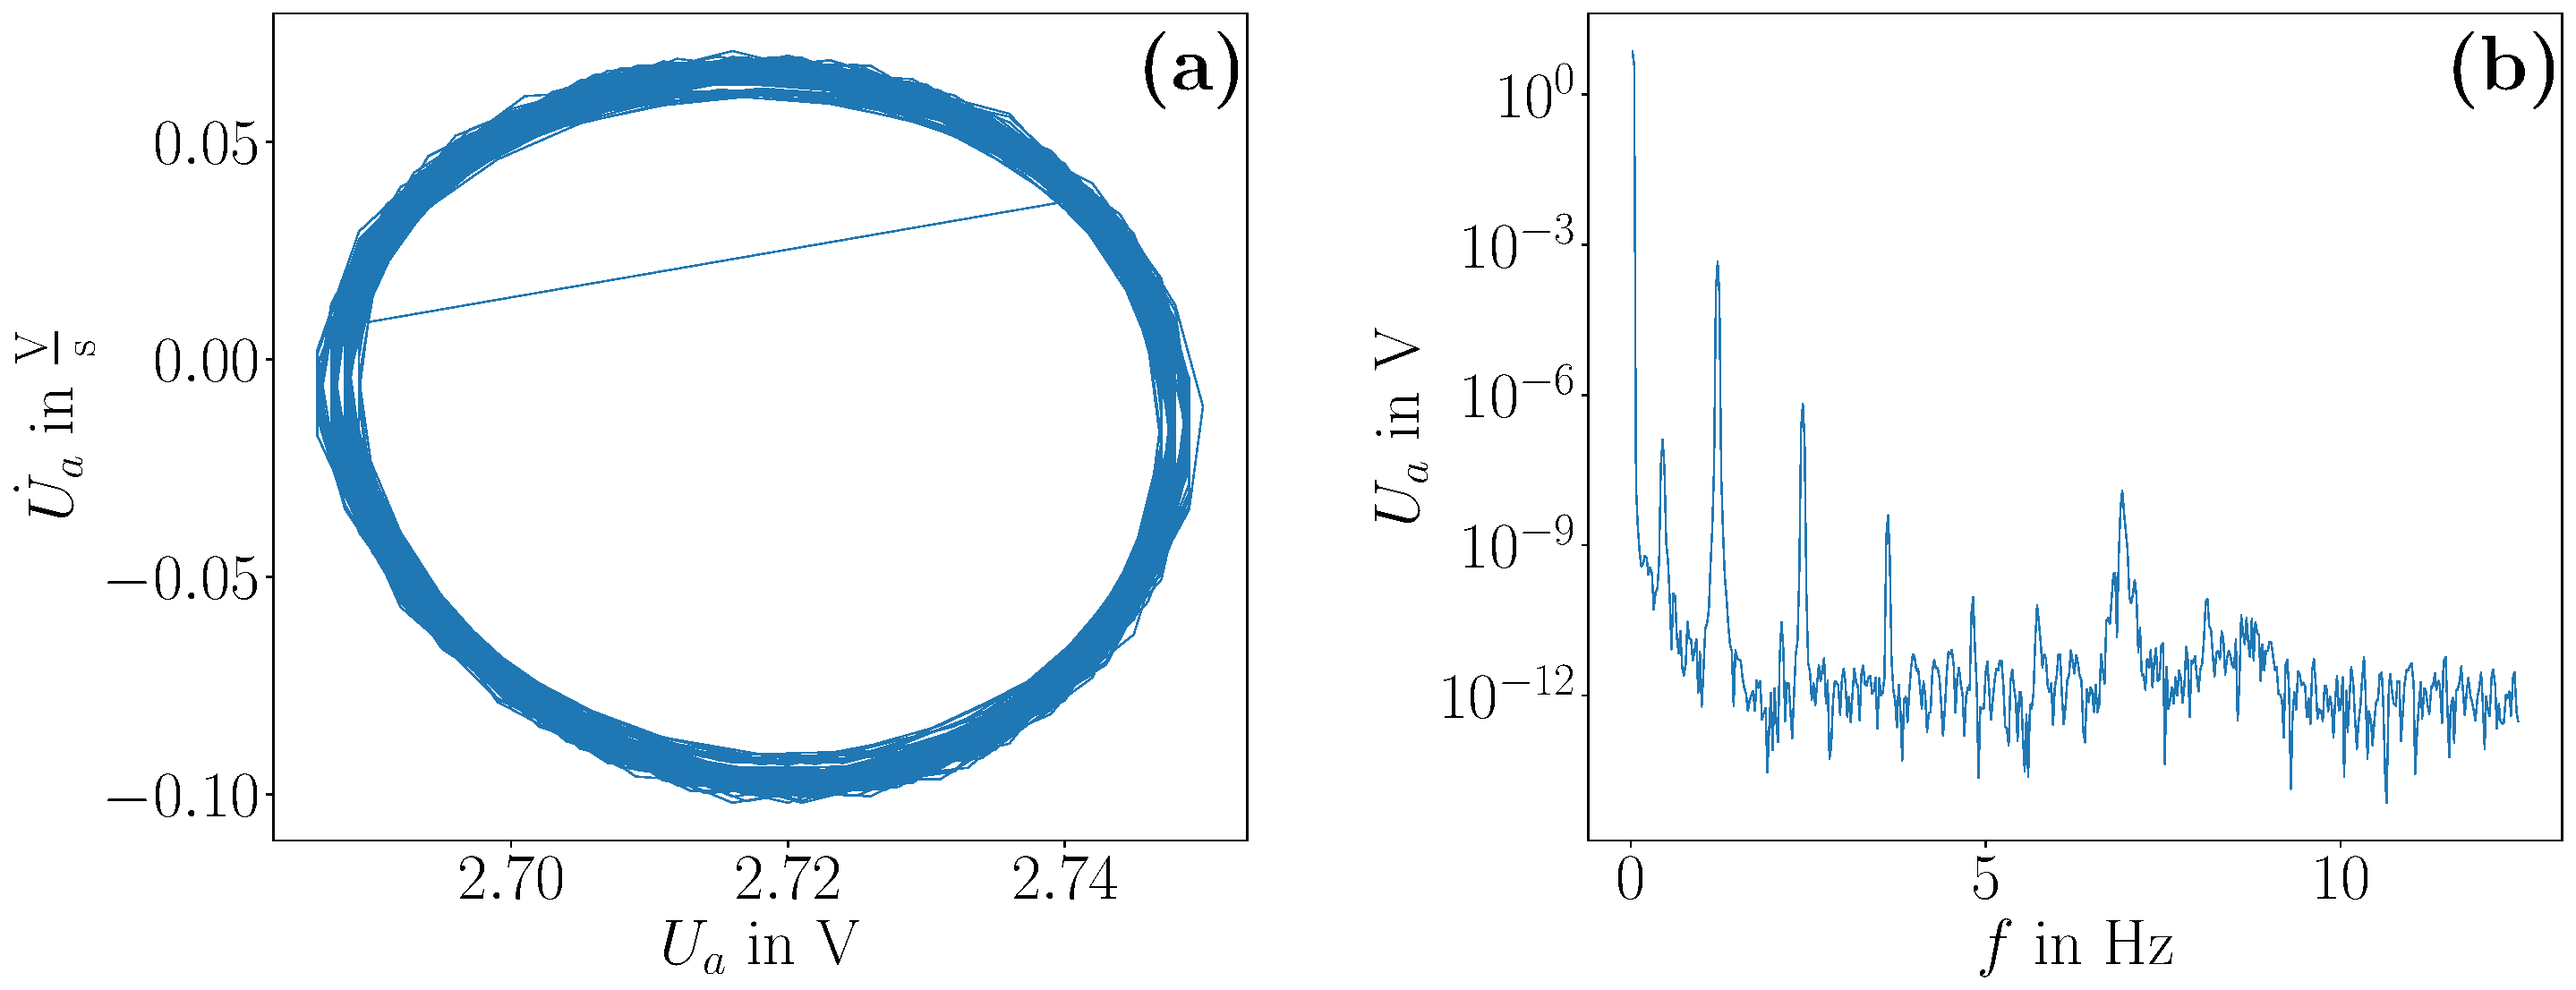
\includegraphics[scale=0.25]{Pendel/3.3a/1,201Hz.pdf}
    \captionof{figure}{Messung bei $f_a$=1,201 Hz, (a) Phasenportrait (b) Leistungsspektrum}
    \label{image:1,201hz}
\end{center}
%\begin{center}
%    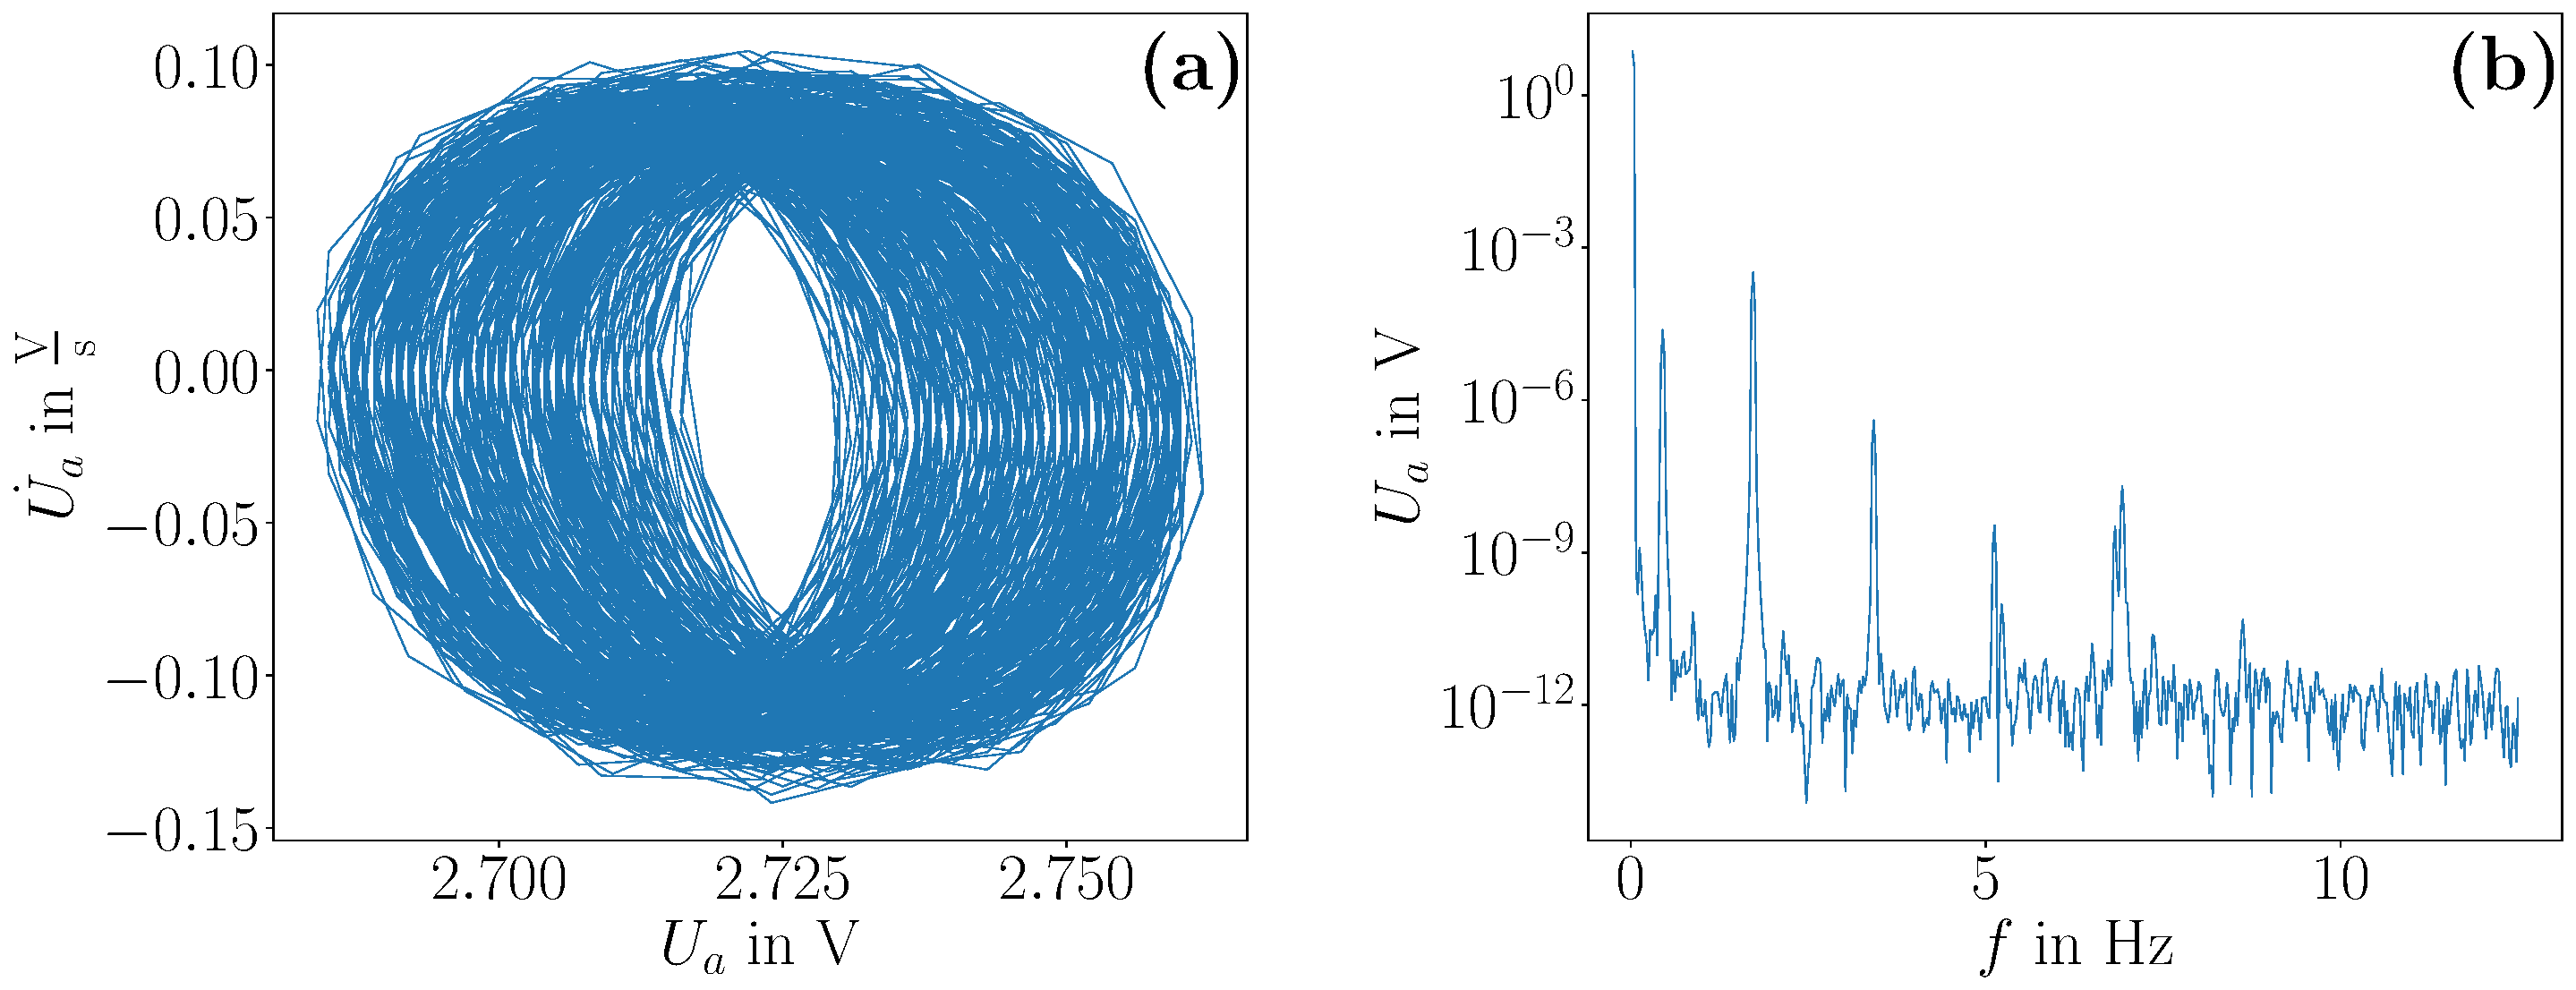
\includegraphics[scale=0.25]{Pendel/3.3a/1,702Hz.pdf}
%    \captionof{figure}{Messung bei $f_a$=1,702 Hz, (a) Phasenportrait (b) Leistungsspektrum}
%    \label{image:1,702hz}
%\end{center}
%\begin{center}
%    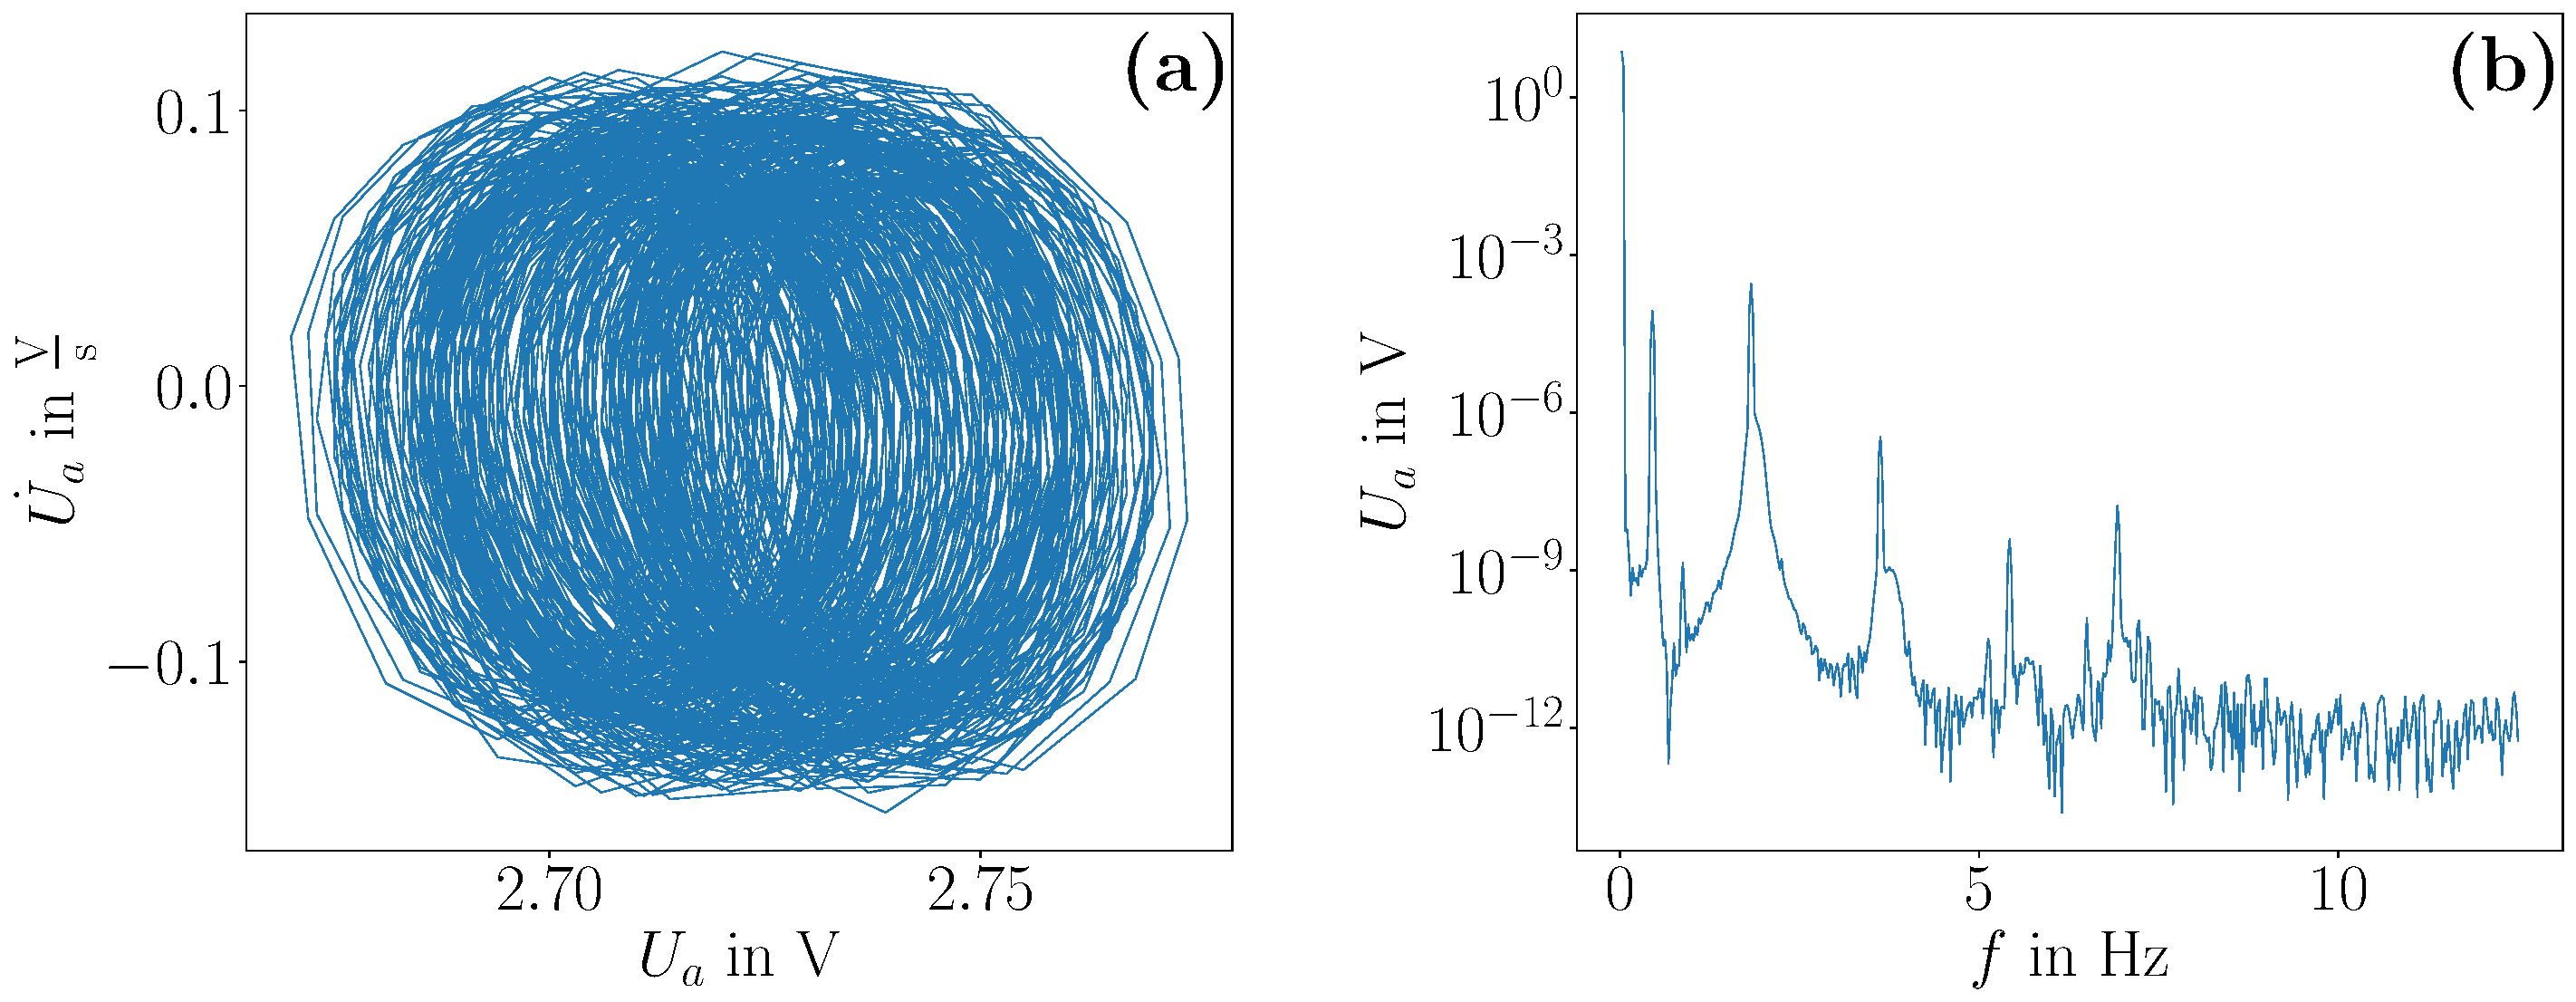
\includegraphics[scale=0.25]{Pendel/3.3a/1,802Hz.pdf}
%    \captionof{figure}{Messung bei $f_a$=1,802 Hz, (a) Phasenportrait (b) Leistungsspektrum}
%    \label{image:1,802hz}
%\end{center}
Ausprägen des Torusattraktors in Abb. \ref{image:2,100hz} bei hoher Frequenzen, mit stark ausgeprägten Peaks im Leistungsspektrum, was für den klar definierten Attraktor spricht.
\begin{center}
    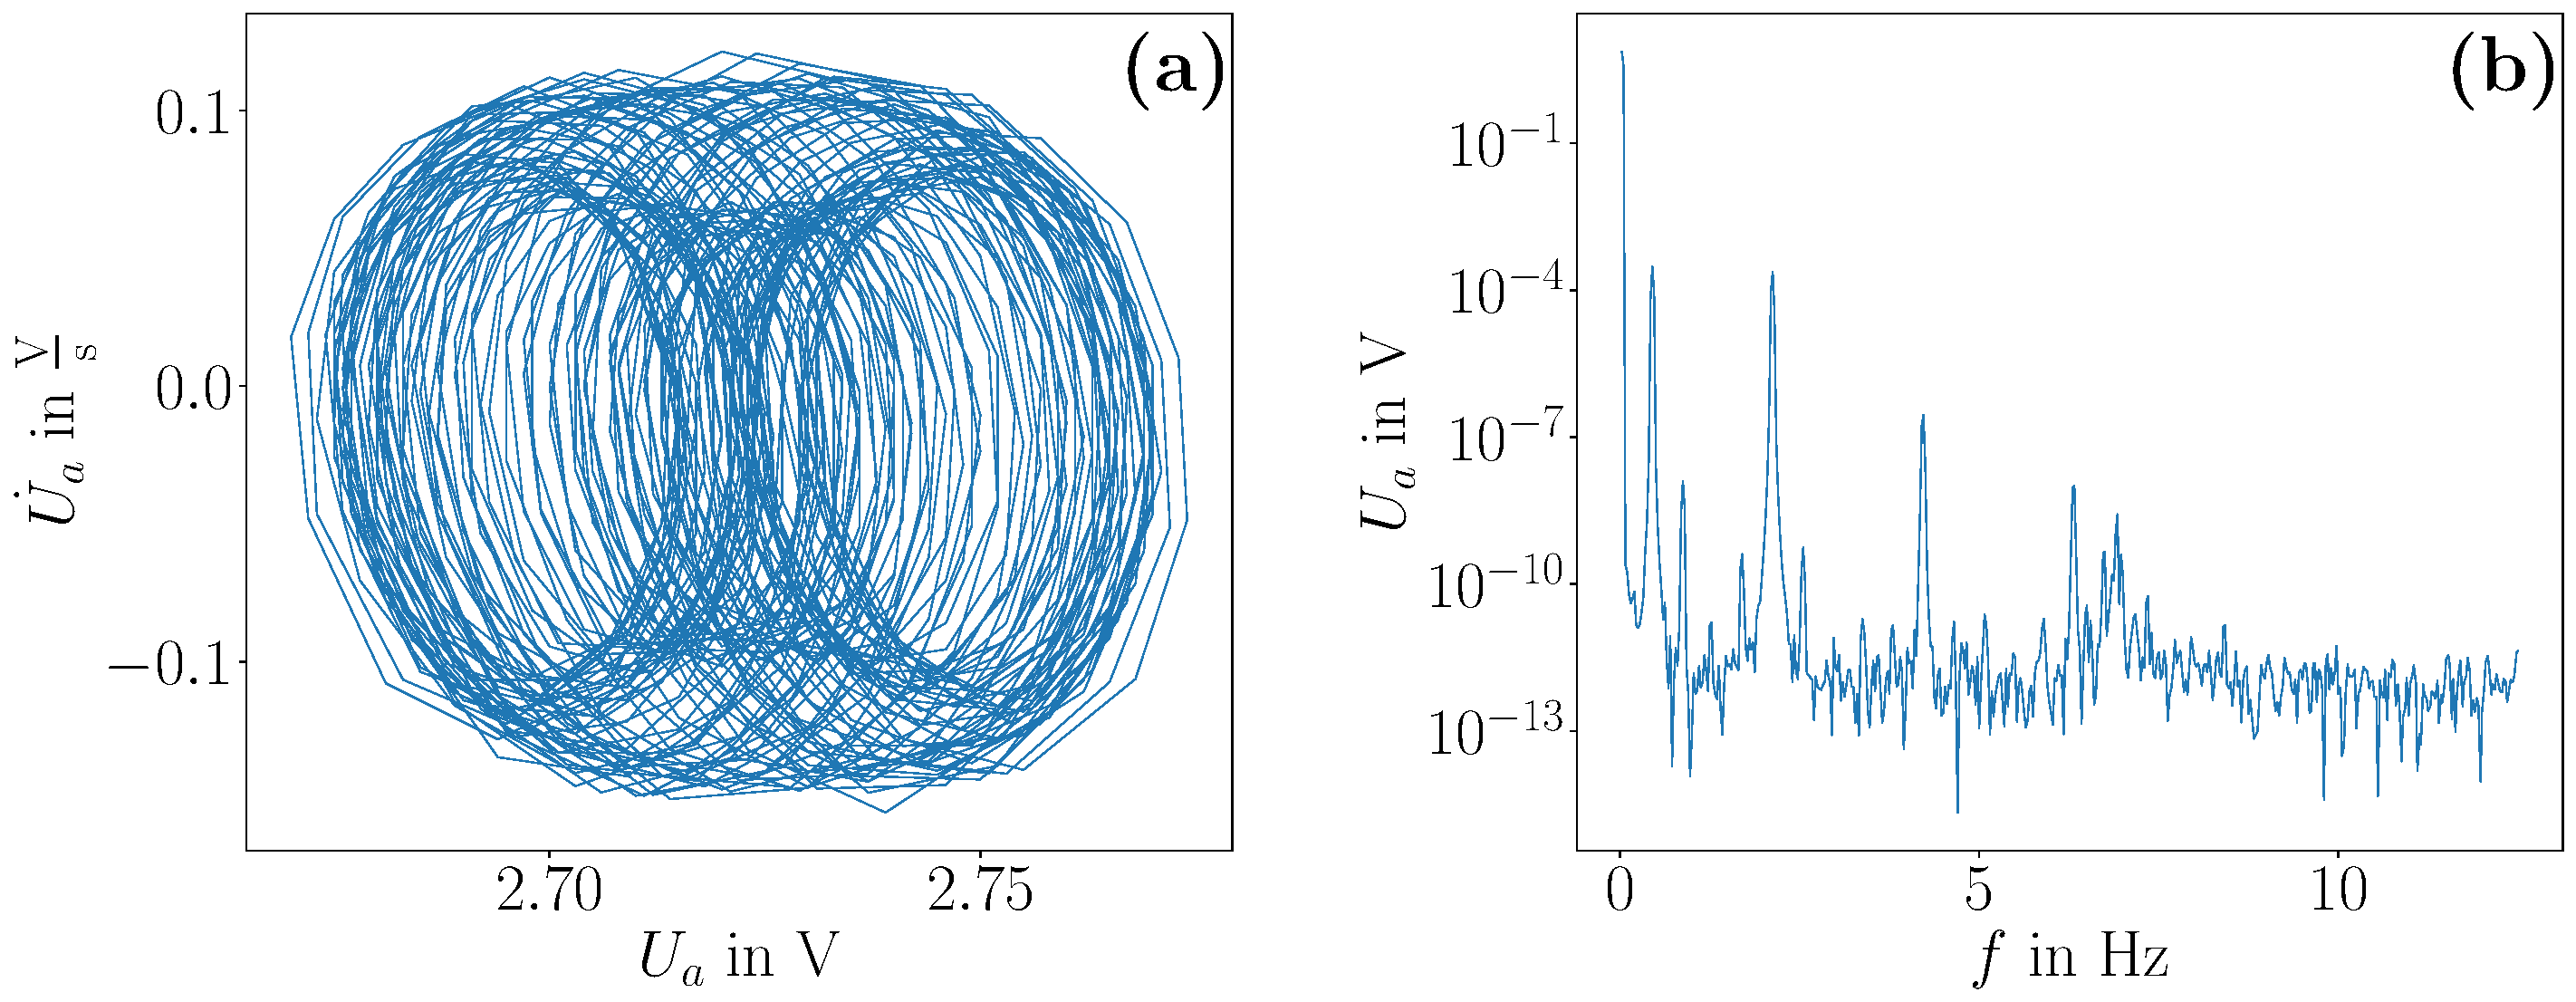
\includegraphics[scale=0.25]{Pendel/3.3a/2,100Hz.pdf}
    \captionof{figure}{Messung bei $f_a$=2,100 Hz, (a) Phasenportrait (b) Leistungsspektrum}
    \label{image:2,100hz}
\end{center}
\newpage
\paragraph{b)} \textbf{Abhängigkeit der Anfangsbedingung}\\
\begin{center}
    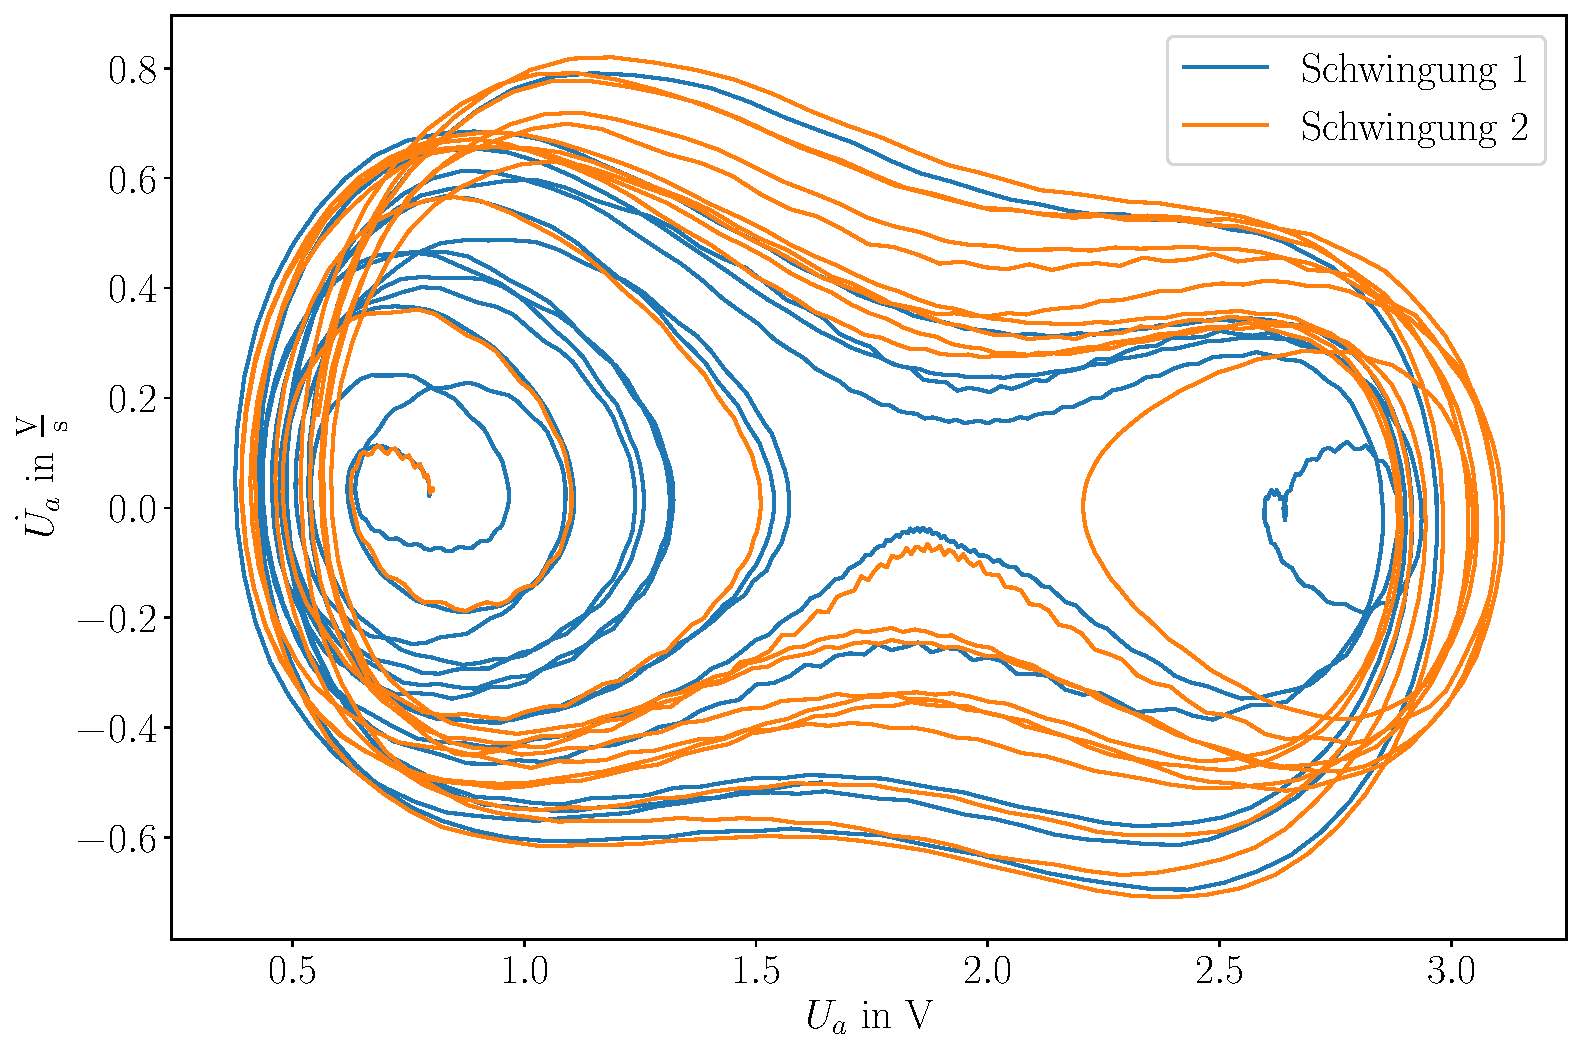
\includegraphics[scale=0.45]{Pendel/3.3b/Schwingungall.pdf}
    \captionof{figure}{Schwingung nach $\Delta T = \SI{56,28}{\sec}$}
    \label{image:allData}
\end{center}
\begin{center}
    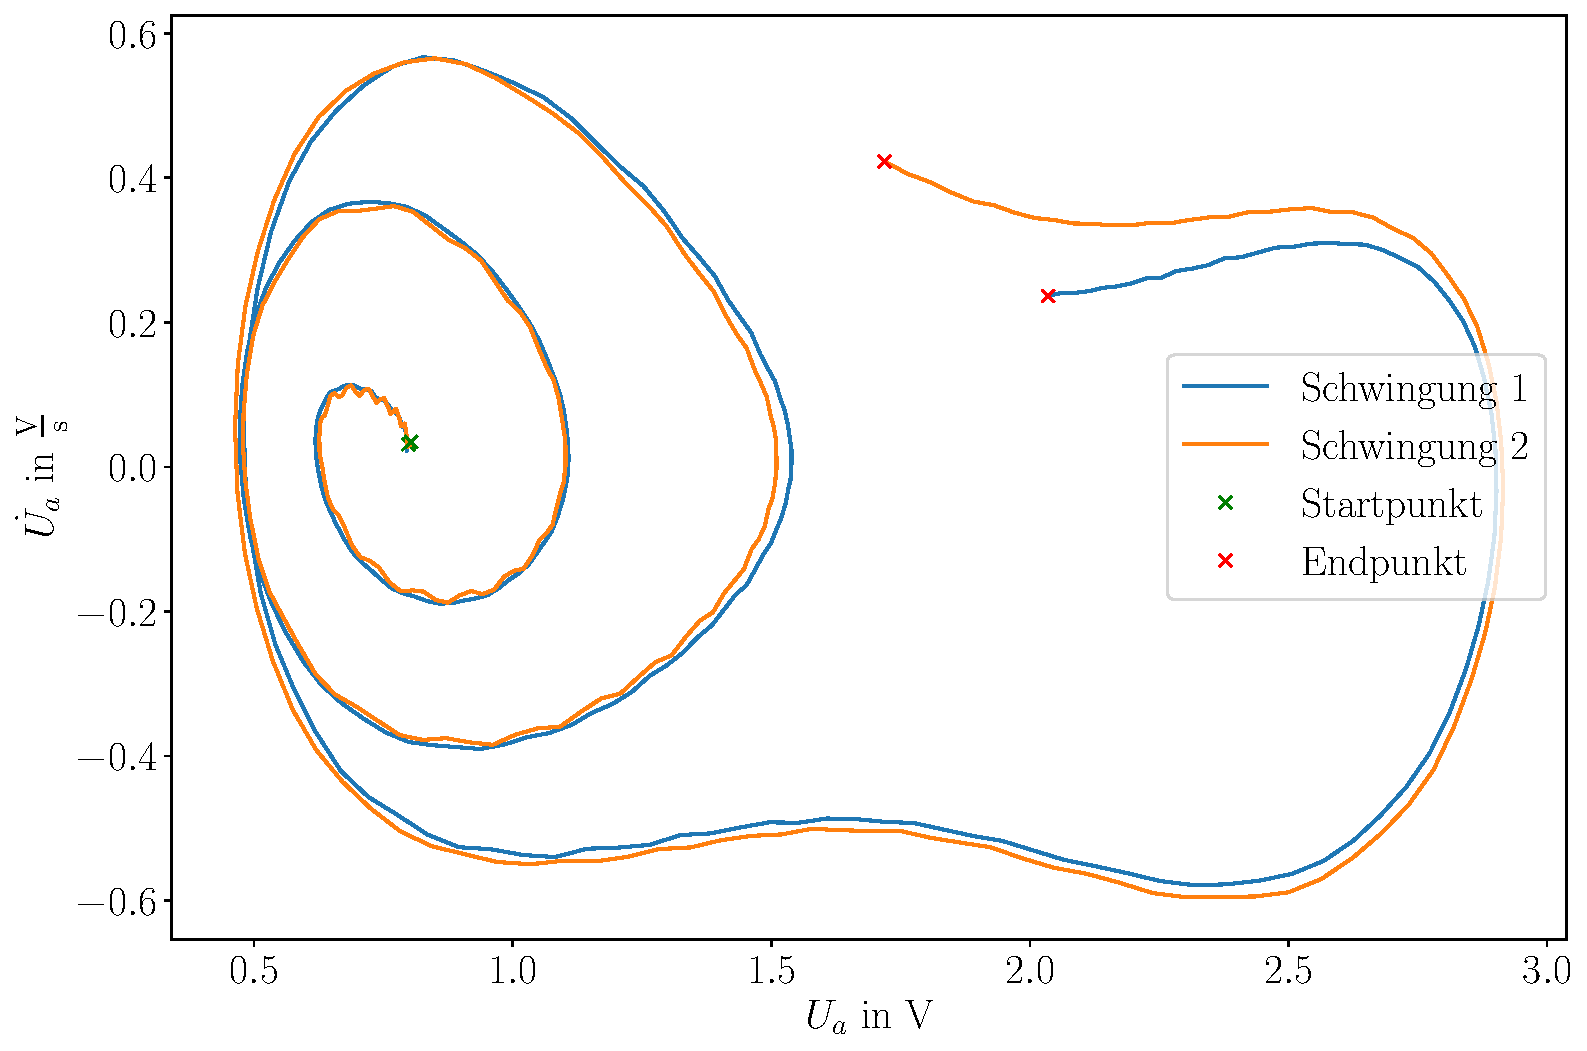
\includegraphics[scale=0.45]{Pendel/3.3b/Startwert.pdf}
    \captionof{figure}{Schwingung mit Start und Endpunkt nach $\Delta T = \SI{10,28}{\sec}$}
    \label{image:startwert}
\end{center}
In Abbildung \ref{image:startwert} erkennt man dann deutlich, dass die Schwingungen sich beim zweiten Umschlag auf die linken Seite voneinander unterscheiden. 